\chapter{Studio di strutture proteiche}
Si è interessati a studiare gli effetti delle deformazioni della struttura proteica sull'entanglement della proteina. In particolare si vuole monitorare come varia il valore dell'entanglement gaussiano, calcolato fra due porzioni della catena, al deformarsi della struttura. 
A tale scopo si è applicata l'analisi ai modi normali con modello anisotropo per lo studio delle proteine 2hqx e 3cry, selezionate fra quelle che presentano un notevole grado di entanglement.
Si sono inoltre osservati gli effetti ottenuti aumentando il valore della costante elastica fra i residui terminali di loop selezionati come quelli maggiormente coinvolti nell'entanglement della struttura, in quanto l'analisi di questi contatti risulta interessante per comprendere il processo di ripiegamento. L'intensità di questi e la fase del processo di ripiegamento in cui si instaurano possono infatti essere cruciali; se questi, ad esempio, dovessero venirsi a creare troppo precocemente potrebbero compromettere il corretto ripiegamento della struttura. \cite{preprint}

\section{Analisi di 2hqx} 
Si è analizzata in primo luogo la proteina 2hqx che è una proteina umana composta da due catene polipeptidiche, A e B, e tra queste si è selezionata la catena A, composta da 86 residui. Si sono reperite le coordinate spaziali dell'atomo di carbonio $ \mathrm{C}^{\alpha} $ di ogni residuo nel Protein Data Bank, dove sono riportate in \AA. Da questo si sono estratti anche i coefficienti B-factor, associati ad ogni atomo e riportati in \AA$^2$, che indicano il grado di mobilità dei singoli atomi ricavato sperimentalmente dal cristallografo. 

Si noti che di seguito per indicare il carbonio $ \mathrm{C}^{\alpha} $ di un residuo ci si riferirà per brevità al residuo stesso. Si tenga inoltre in considerazione che nella numerazione dei modi e dei residui al primo elemento è stato associato l'indice zero.

A partire dalle coordinate spaziali degli atomi $ \mathrm{C}^{\alpha} $ e dalle equazioni (\ref{eq:sub_mat}) e (\ref{eq:sub_mat_diag}), si è calcolata la matrice $ \mathbf{H} $. Qualora la distanza tra i due residui risultasse maggiore del valore scelto per il raggio di cutoff,  $ r_{c} = 18 $ \AA, si è assegnato un valore nullo alla costante elastica. A questa si è invece attribuito valore unitario\footnote{L'effettivo valore della costante elastica risulta in pratica determinato dalla procedura di normalizzazione utilizzata in Figura~\ref{fig:mob_1} per confrontare le mobilità teoriche con i B-factor sperimentali.} 
per residui a distanza inferiore del raggio di cutoff con l'eccezione dei residui consecutivi per i quali si è scelto un valore dieci volte maggiore. In questo modo si è tenuta in considerazione la forza del legame peptidico. 
Una volta ottenuta la matrice si è proceduto con il calcolo degli autovalori e autovettori. Ordinando gli autovalori in modo crescente si vede che i primi sei risultano notevolmente più piccoli degli altri, dell'ordine di $ 10^{-14} $ e $ 10^{-15} $, e corrispondono ai sei autovalori nulli attesi. 

Al fine di ottenere il profilo di mobilità della proteina, si è calcolato il coefficiente di mobilità $ m $ per ogni residuo a partire dall'equazione (\ref{eq:mob}) come 
\begin{equation}
	m_i = \sum_{k=6}^{N} (\Delta \mathbf{R}_i)^2 \bigg|_k
\end{equation} 
dove si è fatta partire la sommatoria dal primo modo con autovalore non nullo. Si sono quindi confrontati graficamente i dati sperimentali con quelli calcolati, sovrapponendo in Figura~\ref{fig:mob_1} i B-factor con i valori di $ m $ dopo aver effettuato un'opportuna normalizzazione di quest'ultimi. Osservando il grafico in Figura~\ref{fig:mob_1} si vede che il profilo di mobilità calcolato segue in modo soddisfacente il dato sperimentale. Si è poi verificato che i risultati fossero stabili al variare del raggio di cutoff. In Figura~\ref{fig:mob_2} si sono quindi riportati i profili di mobilità ottenuti impostando $ r_{c} = 12, \, 14 , \, 16 , \, 18 , \,20$ \AA. È possibile verificare che la variazione del raggio di cutoff attorno al valore $ r_{c} =  18 $ \AA, indicato in letteratura come ottimale per il modello anisotropo, non comporta variazioni significative dei profili di mobilità. \cite{chem_rev}  Si è quindi scelto di procedere con il valore del raggio di cutoff precedentemente scelto in quanto produce il profilo di mobilità che più si avvicina ai dati sperimentali. 
Si sono calcolati infine i gradi di collettività $ \kappa_k $ come indicato nell'equazione (\ref{eq:grado_coll}) per i modi con autovalore non nullo e si sono riportati i risultati in Figura~\ref{fig:gr_coll}.

Si è quindi considerato l'entanglement della proteina. Come si può vedere in Figura~\ref{fig:2hqx}, questa presenta un loop che ha per estremi i residui 10 e 39 all'interno del quale passa un'altra parte di catena della quale si prendono in considerazione la porzione 40-78 che non forma un loop e le porzioni 42-80 e 42-75 che invece costituiscono a loro volta un loop. Si sono scelte queste coppie di sottocatene in quanto (10-39,40-78) è la coppia di sottocatene (di cui solo una è aperta) per cui il valore di $ \lvert G'\rvert $ risulta massimo, (10-39,42-80) è invece la coppia di sottocatene chiuse per cui $ \lvert G'\rvert $ risulta massimo e (10-39,42-75) è la coppia di sottocatene chiuse contenute in (10-39,40-78) per cui $ \lvert G'\rvert $ è massimo.
Al fine di misurare l'entanglement fra queste porzioni della catena si è calcolato l'entanglement gaussiano come prescritto dall'equazione (\ref{eq:link_disc}) e si sono ottenuti i seguenti valori: $ G' $~(10-39,40-78) $ = -1.240 $, $ G' $~(10-39,42-80) $ = -1.010 $ e $ G' $~(10-39,42-75) $ = -0.896 $.
\begin{figure}[h]
	\centering
	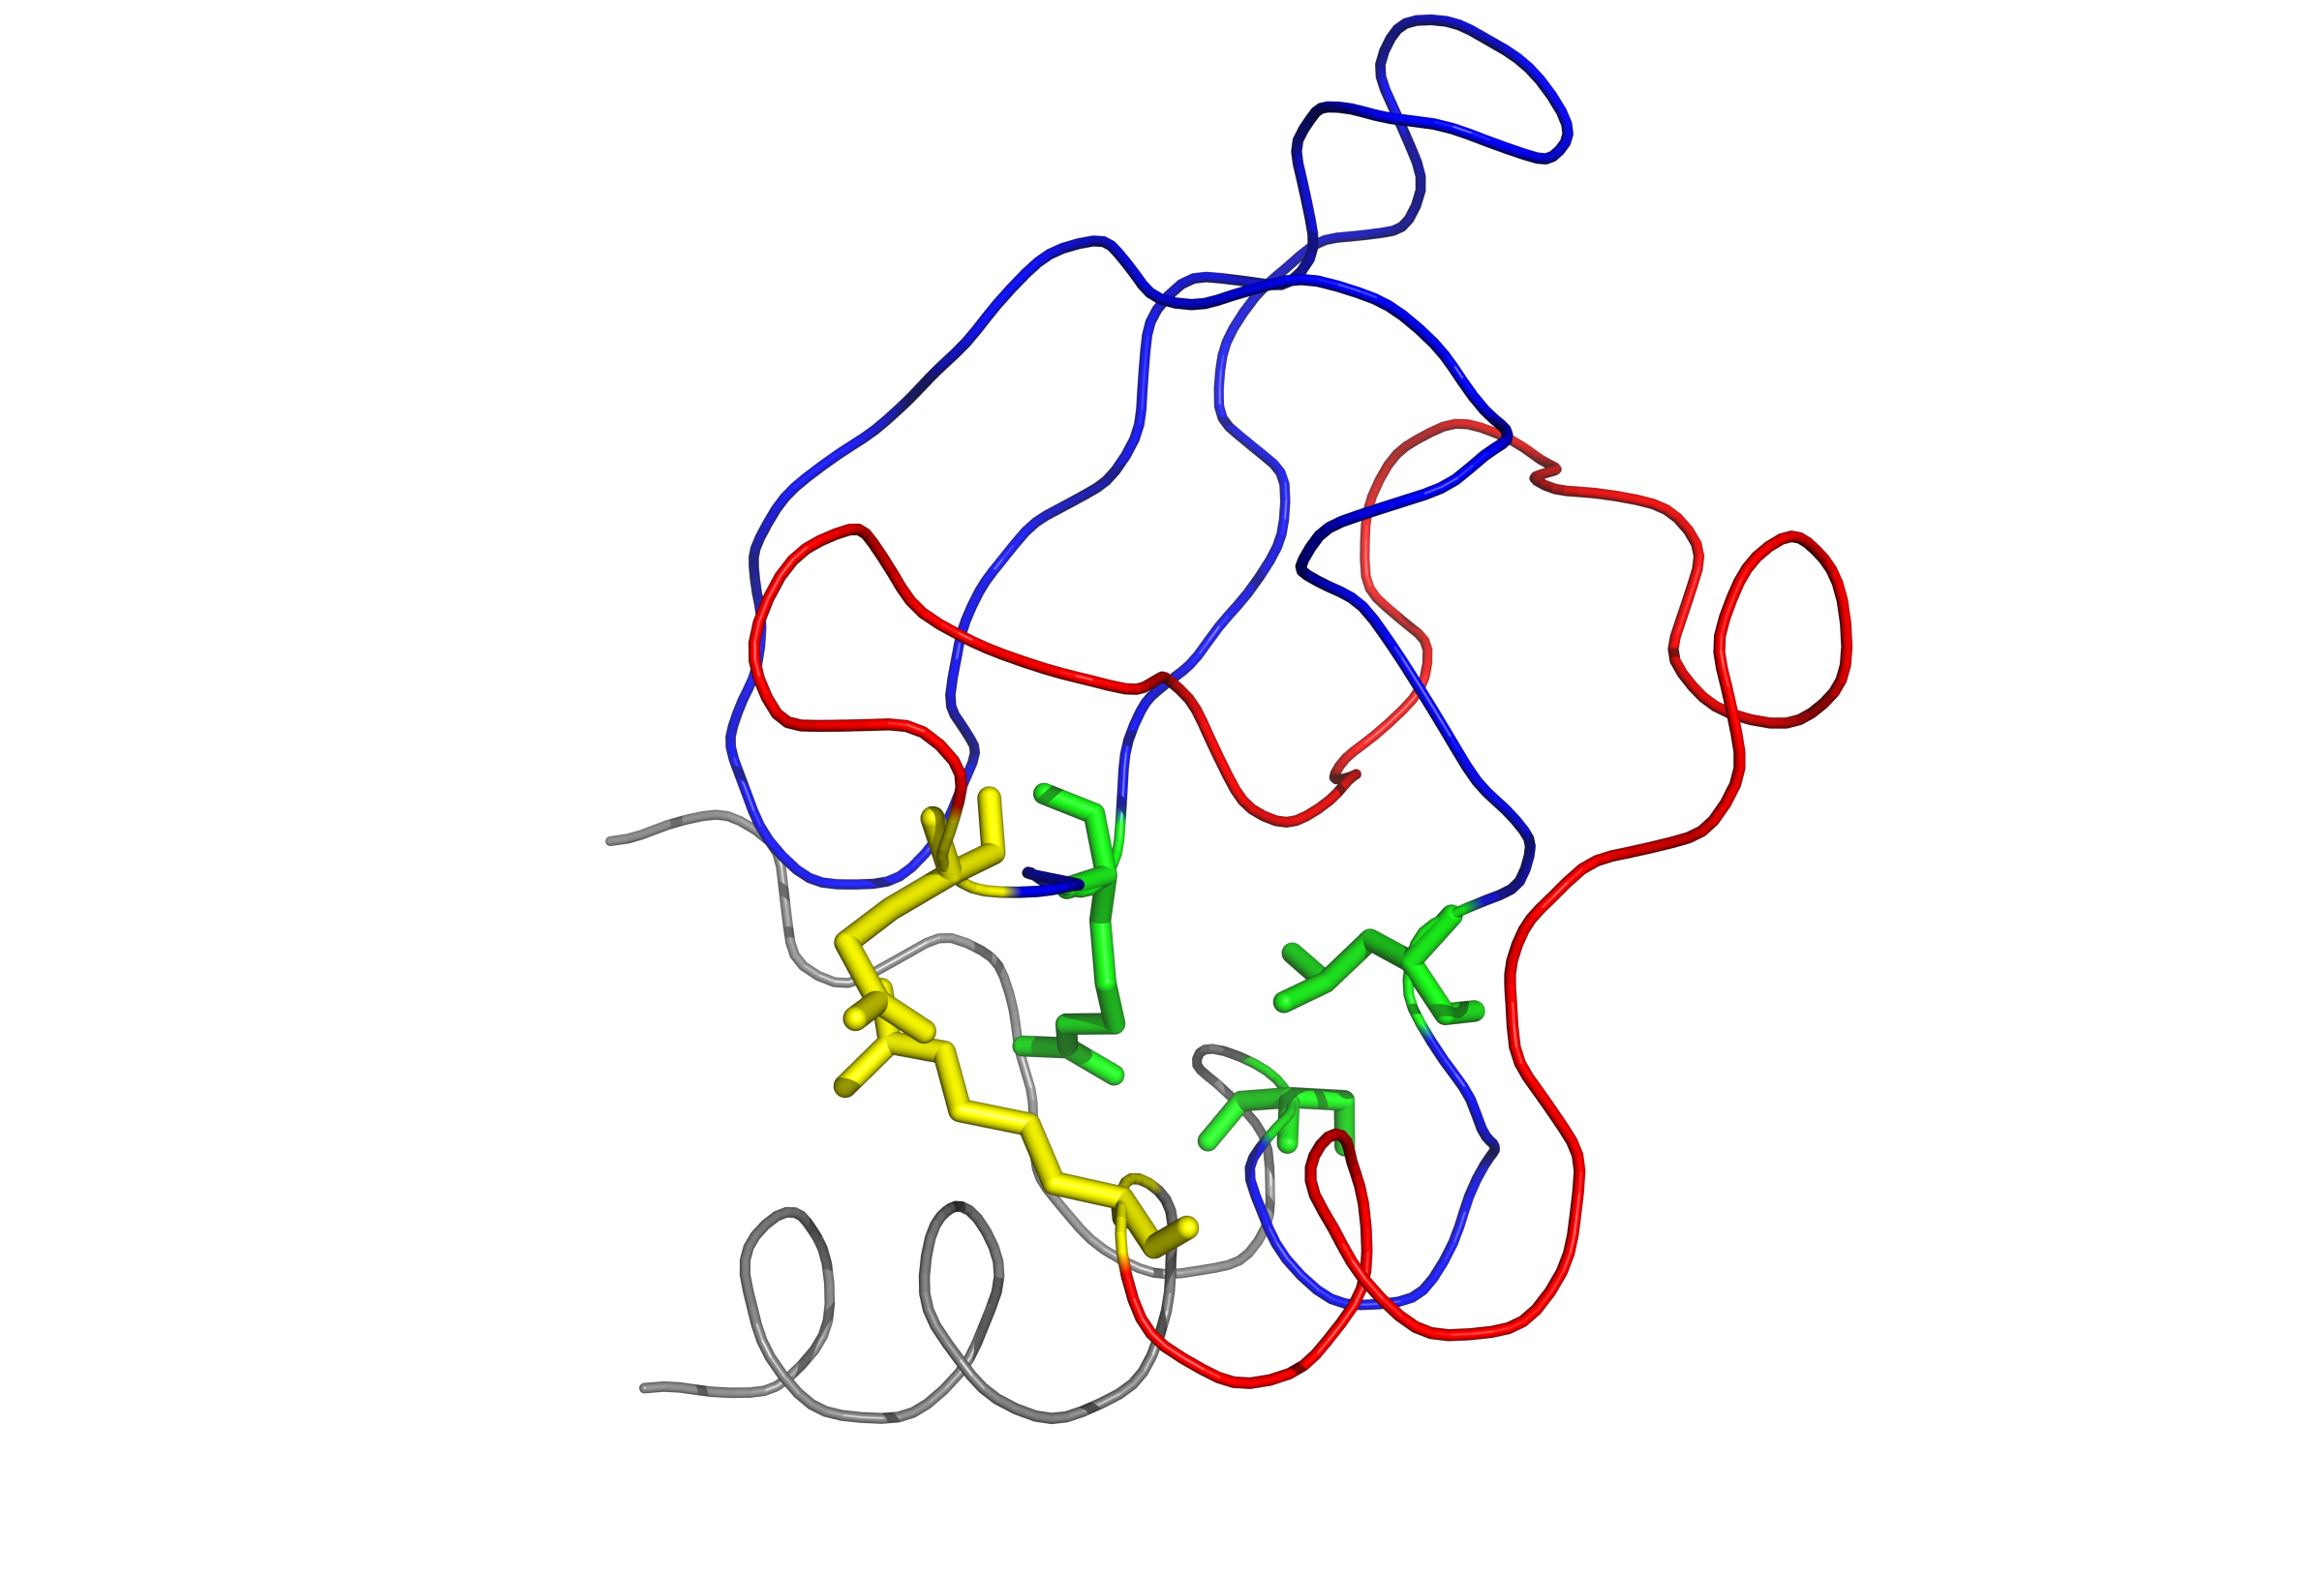
\includegraphics[width=14cm]{/home/michele_puppin/Scrivania/stesura_tesi/immagini/2hqx.png}
	\caption{Raffigurazione delle sottocatene di interesse della catena A di 2hqx. In rosso la catena 10-39 con i residui terminali a contatto in giallo. In blu la catena 40-80 con i residui a contatto 42, 75 e 80 in verde.}
	\label{fig:2hqx}
\end{figure}

Per scegliere lungo quali modi deformare la proteina si è preso in considerazione il grado di mobilità. Poiché come noto ci si aspetta che i modi lenti siano più collettivi si sono considerati i primi modi non nulli $ k=6, \, 7, \, 8, \, 9, \, 10, \, 11 $ in quanto presentano autovalori più separati degli altri. Tra questi inoltre i modi 8 e 9 hanno il grado di collettività maggiore come si può vedere in Figura~\ref{fig:gr_coll}. Il modo con il più alto grado di collettività in assoluto è il modo 121 che, tuttavia, osservando il suo autovettore, presenta una natura casuale e non particolarmente collettiva come atteso per i modi non lenti. Per un'analisi più approfondita si sono andati a considerate i profili di mobilità separatamente per i primi sei modi non nulli. Si è utilizzata a questo scopo l'equazione (\ref{eq:mob}) a $ k $ fissato e si sono riportati i risultati in Figura~\ref{fig:gr_coll_sing}. È possibile osservare come i modi 6 e 7 mostrino fluttuazioni concentrate sugli estremi, risultando quindi scarsamente collettivi, e il modo 11 risulti invece un modo localizzato. Si sono quindi scelti i modi 8 e 9.

Si sono prodotte le deformazioni lungo questi modi utilizzando l'equazione (\ref{eq:deformation}). Per la scelta di $ s $ si è preso un valore $ s_{max} $ che determinasse una variazione della distanza del residuo con il più elevato coefficiente di mobilità (il 50-esimo come si vede in Figura~\ref{fig:mob_1}) dal centro di massa della proteina di qualche punto percentuale (si è scelto il 10\%) in modo da assicurarsi di lavorare intorno alla configurazione non troppo deformata. Si sono quindi scelti 200 valori di $ s $ equidistribuiti nell'intervallo $ [-s_{max} , s_{max}] $. Per ognuno di questi si è determinato il vettore configurazione deformato e si sono calcolati i valori dell'entanglement gaussiano. 
Si è poi provato a bloccare separatamente gli estremi dei loop in contatto, 10-39, 42-80 e 42-75, assegnando alla molla che li collega una costante elastica pari a quella assegnata al legame peptidico.
I risultati ottenuti sono riportati in Figura~\ref{fig:g1}, Figura~\ref{fig:g2} e Figura~\ref{fig:g3} dove è possibile vedere come varia il valore dell'entanglement gaussiano al variare di $ s $ nei casi senza molla aggiuntiva (indicati con n.m.) e nei casi con molla aggiuntiva (m.) per i due modi scelti. Si sono inoltre monitorate le distanze fra gli estremi dei loop 10-39, 42-80 e 42-75 i valori delle quali al variare di $ s $ nelle differenti configurazioni sono riportati in Figura~\ref{fig:d1}, Figura~\ref{fig:d3} e Figura~\ref{fig:d2}. 

Infine si è osservata la variazione degli autovalori considerati prodotta decuplicando il valore della costante elastica di volta in volta per una differente coppia di residui fra quelle connesse da molle nella rete elastica. Rafforzando la molla si ottiene un irrigidimento della rete elastica che essendo meno mobile presenta autovalori più grandi. La variazione degli autovalori, ottenuta bloccando i contatti terminali degli specifici loop studiati in questo lavoro, risulta in linea con quella prodotta agendo sulle altre coppie di residui.

\section{Analisi di 3cry}
Si è analizzata poi la proteina 3cry che è anch'essa una proteina umana composta da due catene, A e B, delle quali si è selezionata la catena A, composta da 169 residui. Questa presenta un elevato grado di entanglement. 

Si è calcolata la matrice $ \mathbf{H} $, scegliendo in questo caso $ r_{c} = 20$ \AA \, per tener conto del maggior numero di residui di 3cry rispetto a 2hqx, e si è proceduto con l'analisi in modo del tutto analogo a quanto fatto per la proteina precedente. In Figura~\ref{fig:mob_100} e Figura~\ref{fig:gr_coll00} si possono osservare rispettivamente i profili di mobilità, che anche in questo caso presentano una buona concordanza tra il dato calcolato e quello sperimentale, e i gradi di collettività. Per quanto riguarda l'entanglement questa proteina presenta un loop che ha per estremi i residui 51 e 122 all'interno del quale passa un'altra parte di catena della quale si prendono in considerazione la porzione 1-50 che non forma un loop e la porzione 10-50 che invece costituisce a sua volta un loop, come si può vedere in Figura~\ref{fig:3cry}. Anche in questo caso si sono scelte queste coppie di sottocatene poiché sono quelle per cui $ \lvert G'\rvert $ è massimo, in maniera analoga a quanto descritto per 2hqx. Si sono poi calcolati i valori dell'entanglement gaussiano ottenendo: $ G' $~(51-122,1-50) $ = -3.067 $ e $ G' $~(51-122,10-50) $ = -2.239 $.
\begin{figure}[h]
	\centering
	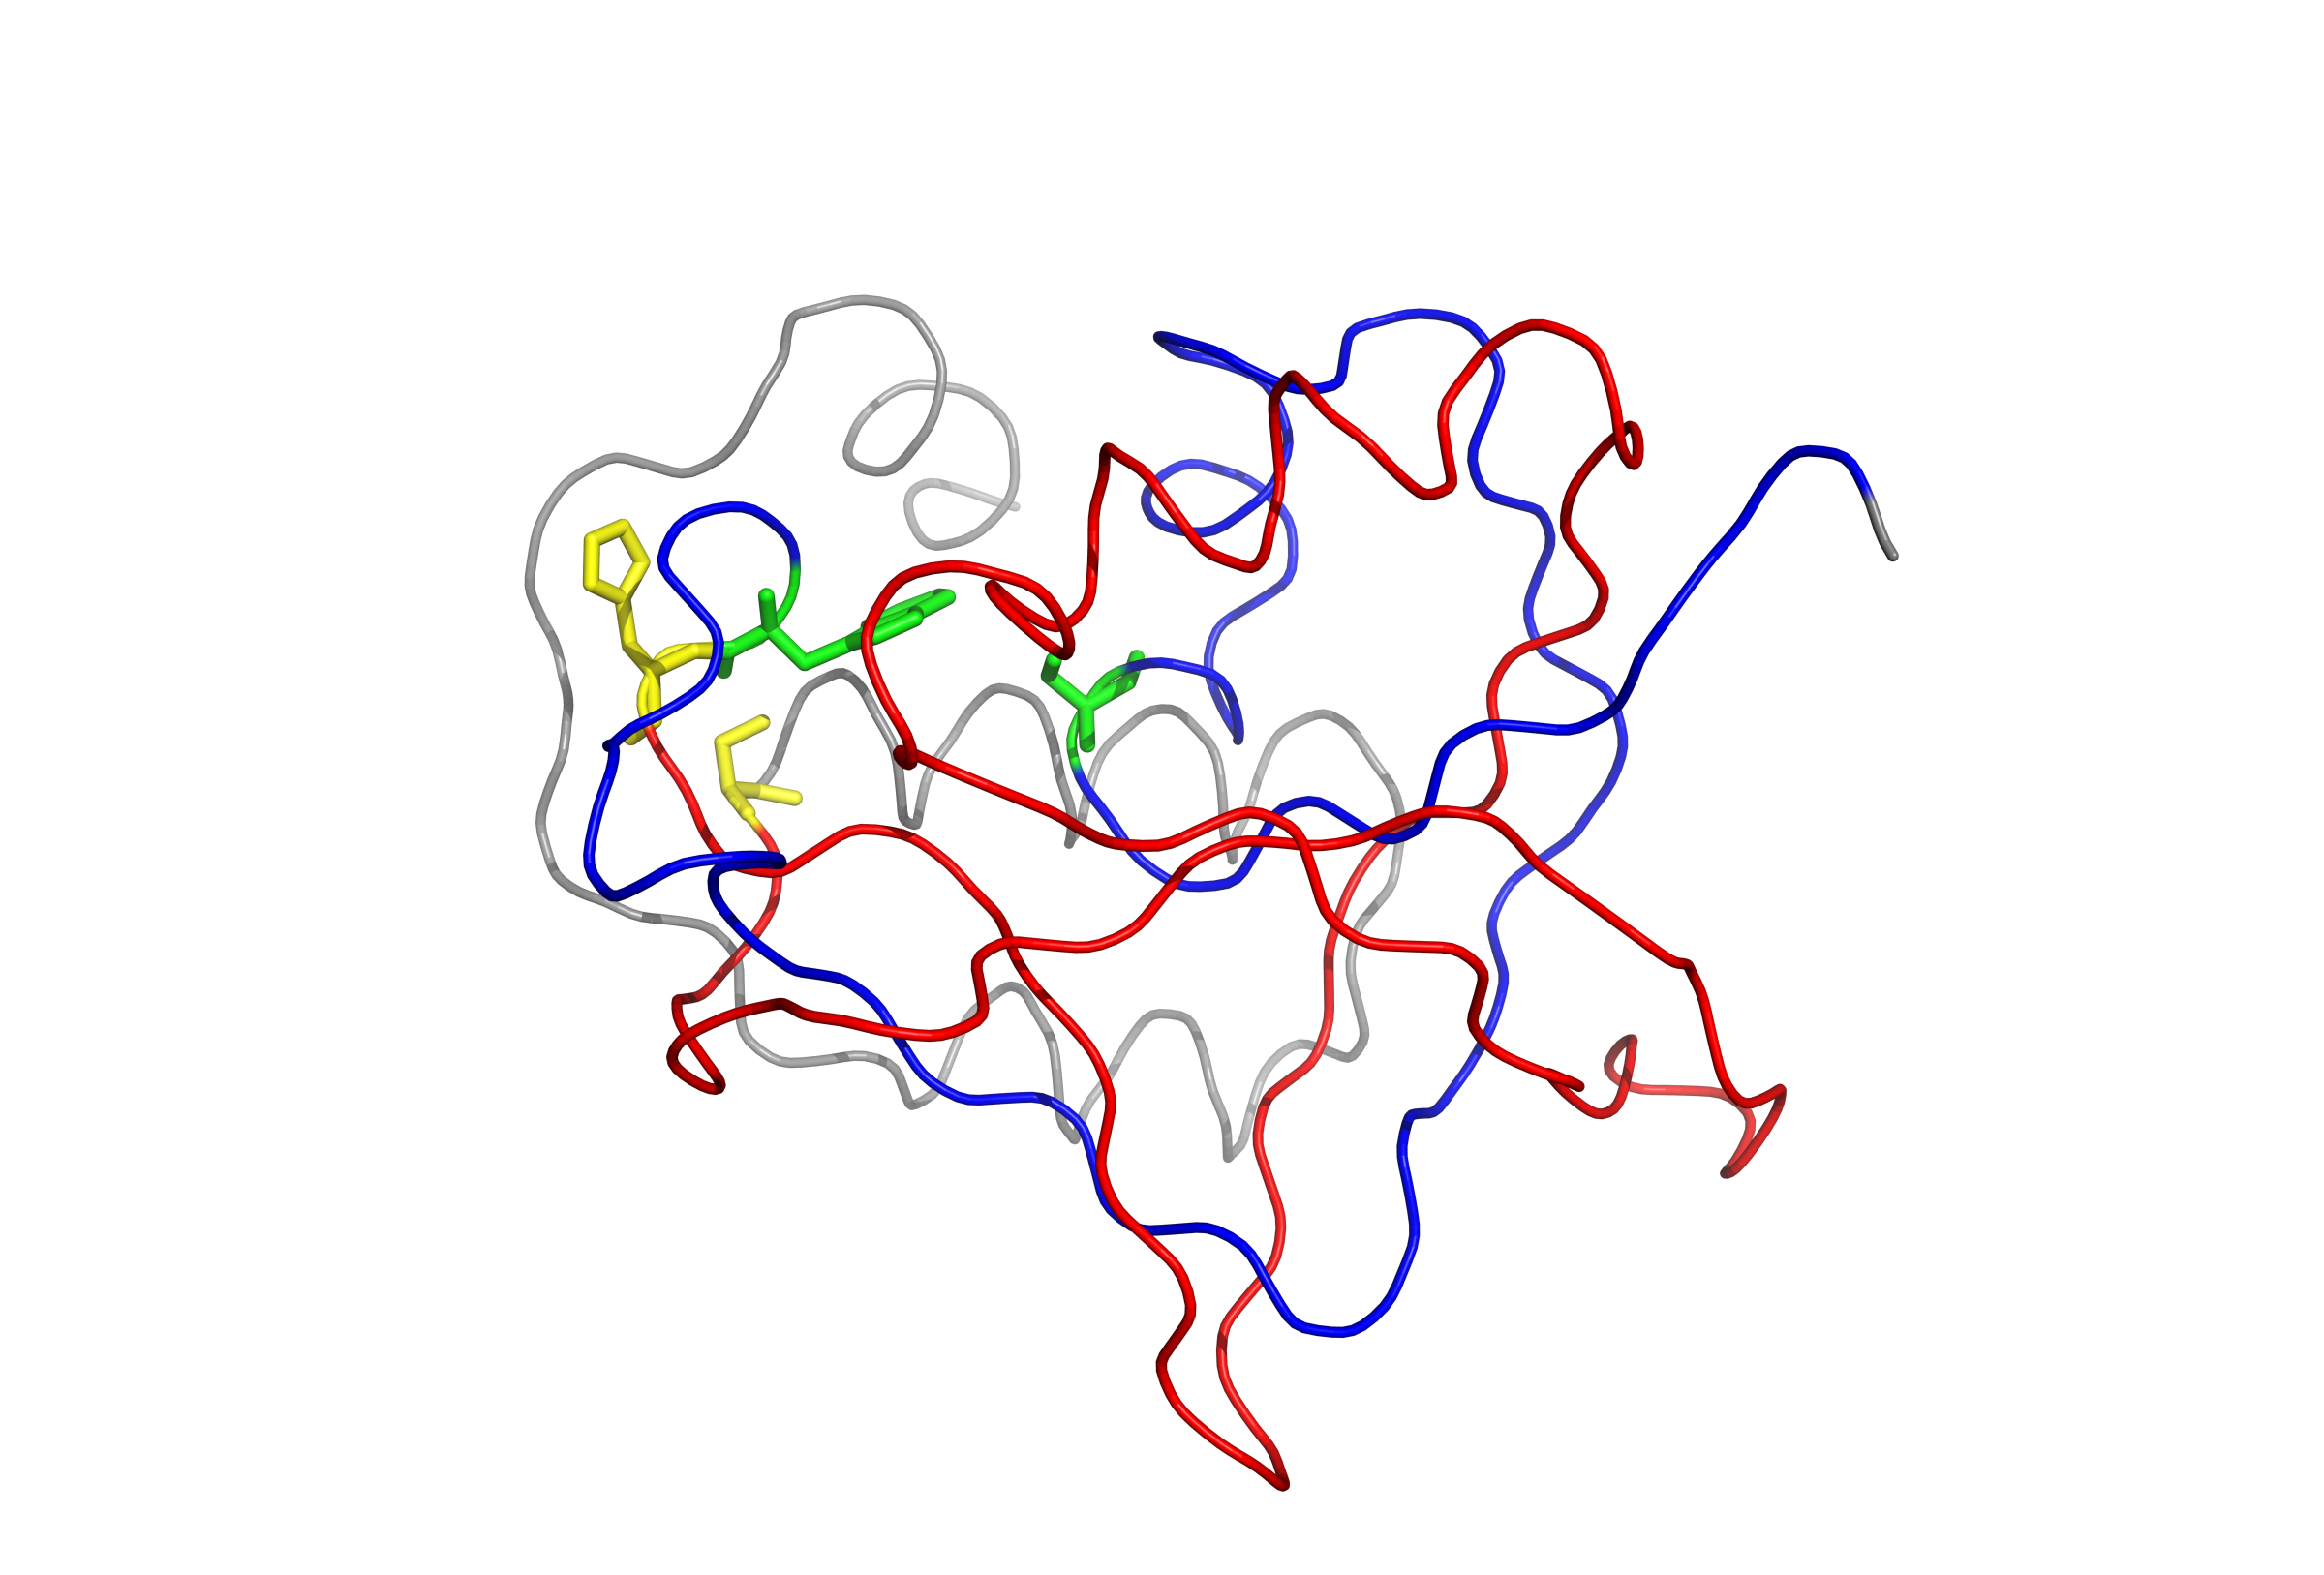
\includegraphics[width=14cm]{/home/michele_puppin/Scrivania/stesura_tesi/immagini/3cry.png}
	\caption{Raffigurazione delle sottocatene di interesse della catena A di 3cry. In rosso la catena 51-122 con i residui terminali a contatto in giallo. In blu la catena 1-50 con i residui a contatto 10 e 50 in verde}
	\label{fig:3cry}
\end{figure}

Per scegliere lungo quali modi deformare la proteina si è preso in considerazione il grado di mobilità con un procedimento analogo a quello per la proteina 2hqx. In questo caso è stato necessario valutare anche i risultati ottenuti eliminando gli ultimi dieci residui. A partire dai B-factor è infatti possibile osservare che questi residui sono dotati di elevata mobilità. Dalla struttura tridimensionale si vede inoltre che questi compongono una $ \alpha $-elica che risulta abbastanza separata dal resto della struttura, eliminandoli risulta quindi più facile individuare i modi di interesse. 
Si sono scelti in questo caso i modi  $ k=7, \, 8, \, 9 $ e lungo questi si sono prodotte le deformazioni. 
Si è inoltre nuovamente proceduto a bloccare gli estremi dei loop in contatto, 51-122 e 10-50.
In Figura~\ref{fig:g100} e Figura~\ref{fig:g200} è possibile osservare l'andamento dei valori dell'entanglement gaussiano per i tre modi scelti e nelle varie configurazioni. L'andamento delle distanze fra gli estremi dei loop può essere invece osservato in Figura~\ref{fig:d100} e Figura~\ref{fig:d200}.

Al fine di confrontare più agevolmente la variazione dei valori dell'entanglement gaussiano e delle distanze se ne sono calcolate le  derivate rispetto al parametro $ s $ che controlla le deformazioni lungo i vari modi. 
Per quanto riguarda $ G' $ si è proceduto con un calcolo numerico considerando la derivata centrata 
\begin{equation}
\frac{\mathrm{d}G'}{\mathrm{d}s} \bigg|_{s=s_0}  = \frac{G'(s_0 + \Delta s) - G'(s_0 - \Delta s)}{2 \Delta s} 
\end{equation}
con $s_0 = 0  $ e $\Delta s = 10^{-5}  $. Si deve quindi calcolare $ G'(\pm \Delta s) $ che è inteso come l'entanglement gaussiano a partire dal vettore configurazione deformato $ \mathbf{q}^{(k)} = \mathbf{q}^0 \pm  \Delta s \lambda_{k}^{-1/2} \mathbf{u}_k$. 
Si è calcolata poi la derivata seconda 
\begin{equation}
\frac{\mathrm{d}^2G'}{\mathrm{d}s^2} \bigg|_{s=s_0}  = \frac{G'(s_0 + \Delta s) + G'(s_0 - \Delta s) - 2 G'(s_0)}{\Delta s^2}.
\end{equation}
Per quanto riguarda invece la distanza fra i residui $  i $ e $ j $ terminali dei un loop si ha che
\begin{equation}
\mathbf{d} (s) =
\left(
\begin{array}{ccc}
q^{0}_{i,x} \\
q^{0}_{i,y} \\
q^{0}_{i,z} \\                       
\end{array}
\right) + s \lambda_{k}^{-1/2}
\left(
\begin{array}{ccc}
u_{k,i,x} \\
u_{k,i,y} \\
u_{k,i,z} \\
\end{array}
\right) - 
\left[
\left(
\begin{array}{ccc}
q^{0}_{j,x} \\
q^{0}_{j,y} \\
q^{0}_{j,z} \\
\end{array}
\right) + s \lambda_{k}^{-1/2}
\left(
\begin{array}{ccc}
u_{k,j,x} \\
u_{k,j,y} \\
u_{k,j,z} \\
\end{array}
\right)
\right]
\end{equation}
Si può quindi scrivere $ \mathbf{d} (s) = \mathbf{a} + s \mathbf{b} $ con
\begin{equation}
\mathbf{a} =
\left(
\begin{array}{ccc}
q^{0}_{i,x} - q^{0}_{j,x}\\
q^{0}_{i,y} - q^{0}_{j,y}\\
q^{0}_{i,z} - q^{0}_{j,z}\\
\end{array}
\right)
\qquad \mathrm{e} \qquad
\mathbf{b} = 
\lambda_{k}^{-1/2}
\left(
\begin{array}{ccc}
u_{k,i,x} - u_{k,j,x}\\
u_{k,i,y} - u_{k,j,y}\\
u_{k,i,z} - u_{k,j,z}\\
\end{array}
\right).
\end{equation}
Si ha quindi che la distanza risulta  $ d(s) = \lVert \mathbf{d} \rVert = \lVert \mathbf{a} + s \mathbf{b} \rVert$ ed è possibile calcolare in modo analitico la derivata prima in zero come
\begin{equation}
d' =  \frac{\mathbf{a} \cdot \mathbf{b}}{ \lVert \mathbf{a} \rVert }
\end{equation}
e la derivata seconda in zero come
\begin{equation}
d'' =  \frac{\lVert \mathbf{b} \rVert^2}{ \lVert \mathbf{a} \rVert } - \frac{ \left( \mathbf{a} \cdot \mathbf{b} \right)^2}{ \lVert\mathbf{a} \rVert^3 }.
\end{equation}
In Tabella~\ref{tb:modo_7}, Tabella~\ref{tb:modo_8} e Tabella~\ref{tb:modo_9} si sono riportati i moduli delle derivate divise per il valore della funzione corrispondente in $ s=0 $ in modo da valutare la variazioni in termini relativi.

\section{Conclusioni}
Dall'analisi dei grafici prodotti e dei valori delle derivate calcolati è possibile osservare come il grado di entanglement rimanga sostanzialmente invariato nelle differenti configurazioni assunte dalla proteina in un intorno dello stato nativo. In tutti i casi infatti i valori di $ \lvert G' \rvert $ variano in un range ristretto rispetto al valore di riferimento. Osservando in particolare i valori delle derivate poi è possibile vedere come il valore dell'entanglement gaussiano sia meno dipendente da s rispetto alle distanze che comunque non variano in modo significativo. 
Si vede quindi che complessivamente le fluttuazioni lungo i modi lenti non inducono variazioni significative sul grado di entanglement della proteina e di conseguenza bloccare i residui a contatto non sortisce particolari effetti. 
L'analisi di altre proteine e l'utilizzo di modelli più sofisticati di rete elastica \cite{md} saranno necessari per confermare questa conclusione in generale.

